Ein Mobile besteht aus zwei leichten Stäben. Am unteren Stab hängt $b_1 = \bLiO$ links von seiner Schnur eine Masse $m_2 = \mKbO$ und $b_2 = \bReO$ rechts davon eine Masse $m_3$. Der untere Stab hängt am rechten Ende des oberen Stabs, im Abstand $x$ von dessen Schnur; $a_1 = \aObO$ links dieser Schnur hängt eine Masse $m_1 = \mKaO$. Bestimme $m_3$ und $x$ so, dass beide Stäbe waagrecht hängen.

\begin{center}
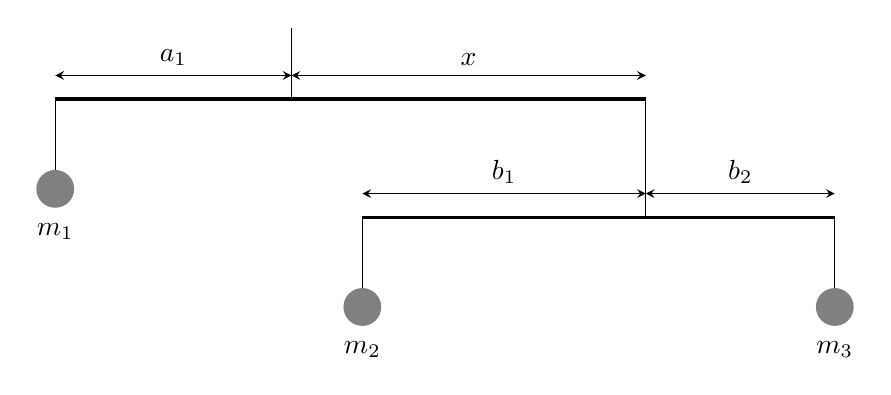
\begin{tikzpicture}[scale=0.3, >=stealth]
 \draw (0,3) -- (0,0);
 \draw[very thick] (-10,0) -- (15,0);
 \draw (-10,0) -- (-10,-3);
 \fill[gray] (-10,-3.8) circle (0.8);
 \node at (-10,-5.6) {$m_1$};
 \draw (15,0) -- (15,-5);
 \draw[very thick] (3,-5) -- (23,-5);
 \draw (3,-5) -- (3,-8);
 \fill[gray] (3,-8.8) circle (0.8);
 \node at (3,-10.6) {$m_2$};
 \draw (23,-5) -- (23,-8);
 \fill[gray] (23,-8.8) circle (0.8);
 \node at (23,-10.6) {$m_3$};
 \draw[<->] (-10,1) -- (0,1) node[midway, above] {$a_1$};
 \draw[<->] (0,1) -- (15,1) node[midway, above] {$x$};
 \draw[<->] (3,-4) -- (15,-4) node[midway, above] {$b_1$};
 \draw[<->] (15,-4) -- (23,-4) node[midway, above] {$b_2$};
\end{tikzpicture}
\end{center}
(Skizze nicht massstäblich.)
